\chapter{Evaluation}
\label{chapter:evaluation}

% \emph{[Deployed model performance evaluation,  Real time prediction tests] }
%  \bigskip

In the following section, the last step of the project development, the testing will be elaborated. Starting from the problem definition, the multisensory solution will be contrasted to the traditional PIR-only light control algorithms in the selected environments. The pilot study involved extensive data collection from all modules to best evaluate and demonstrate the general differences and edge cases in light control behavior.

\section{Test environment}

In the selection of the test environments, the main objective was to identify places where the PIR-based light control solutions notoriously struggle, where there is the most need for alternative approaches. Finding those places and evaluate the effectiveness of the introduction of sound information is key to the viability of the project.

Among company office premises one of the most problematic room types is the private meeting room from an automatic lighting control or presence detection standpoint using traditional PIR sensors. Due to their small size, employees tend to use them for joining a virtual meeting alone or hop in for private phone calls for a short amount of time, so they do not disturb others while having a conversation. Office phone booths have usually one seating place only with limited options for any movement, which makes it hard for PIR sensors to detect motion.

The assembled prototype is then placed in such a private phone booth for testing purposes as it is visible on \autoref{fig:testbox_desk}. From the outside and LED strip indicates the automatic lighting control decisions made by the algorithm based on the audio and PIR measurements discussed earlier. Only the microphone port and the PIR sensor are exposed in the direction of the user, power cords were concealed in the back of the device.


\begin{figure}[t!]
  \begin{center}
    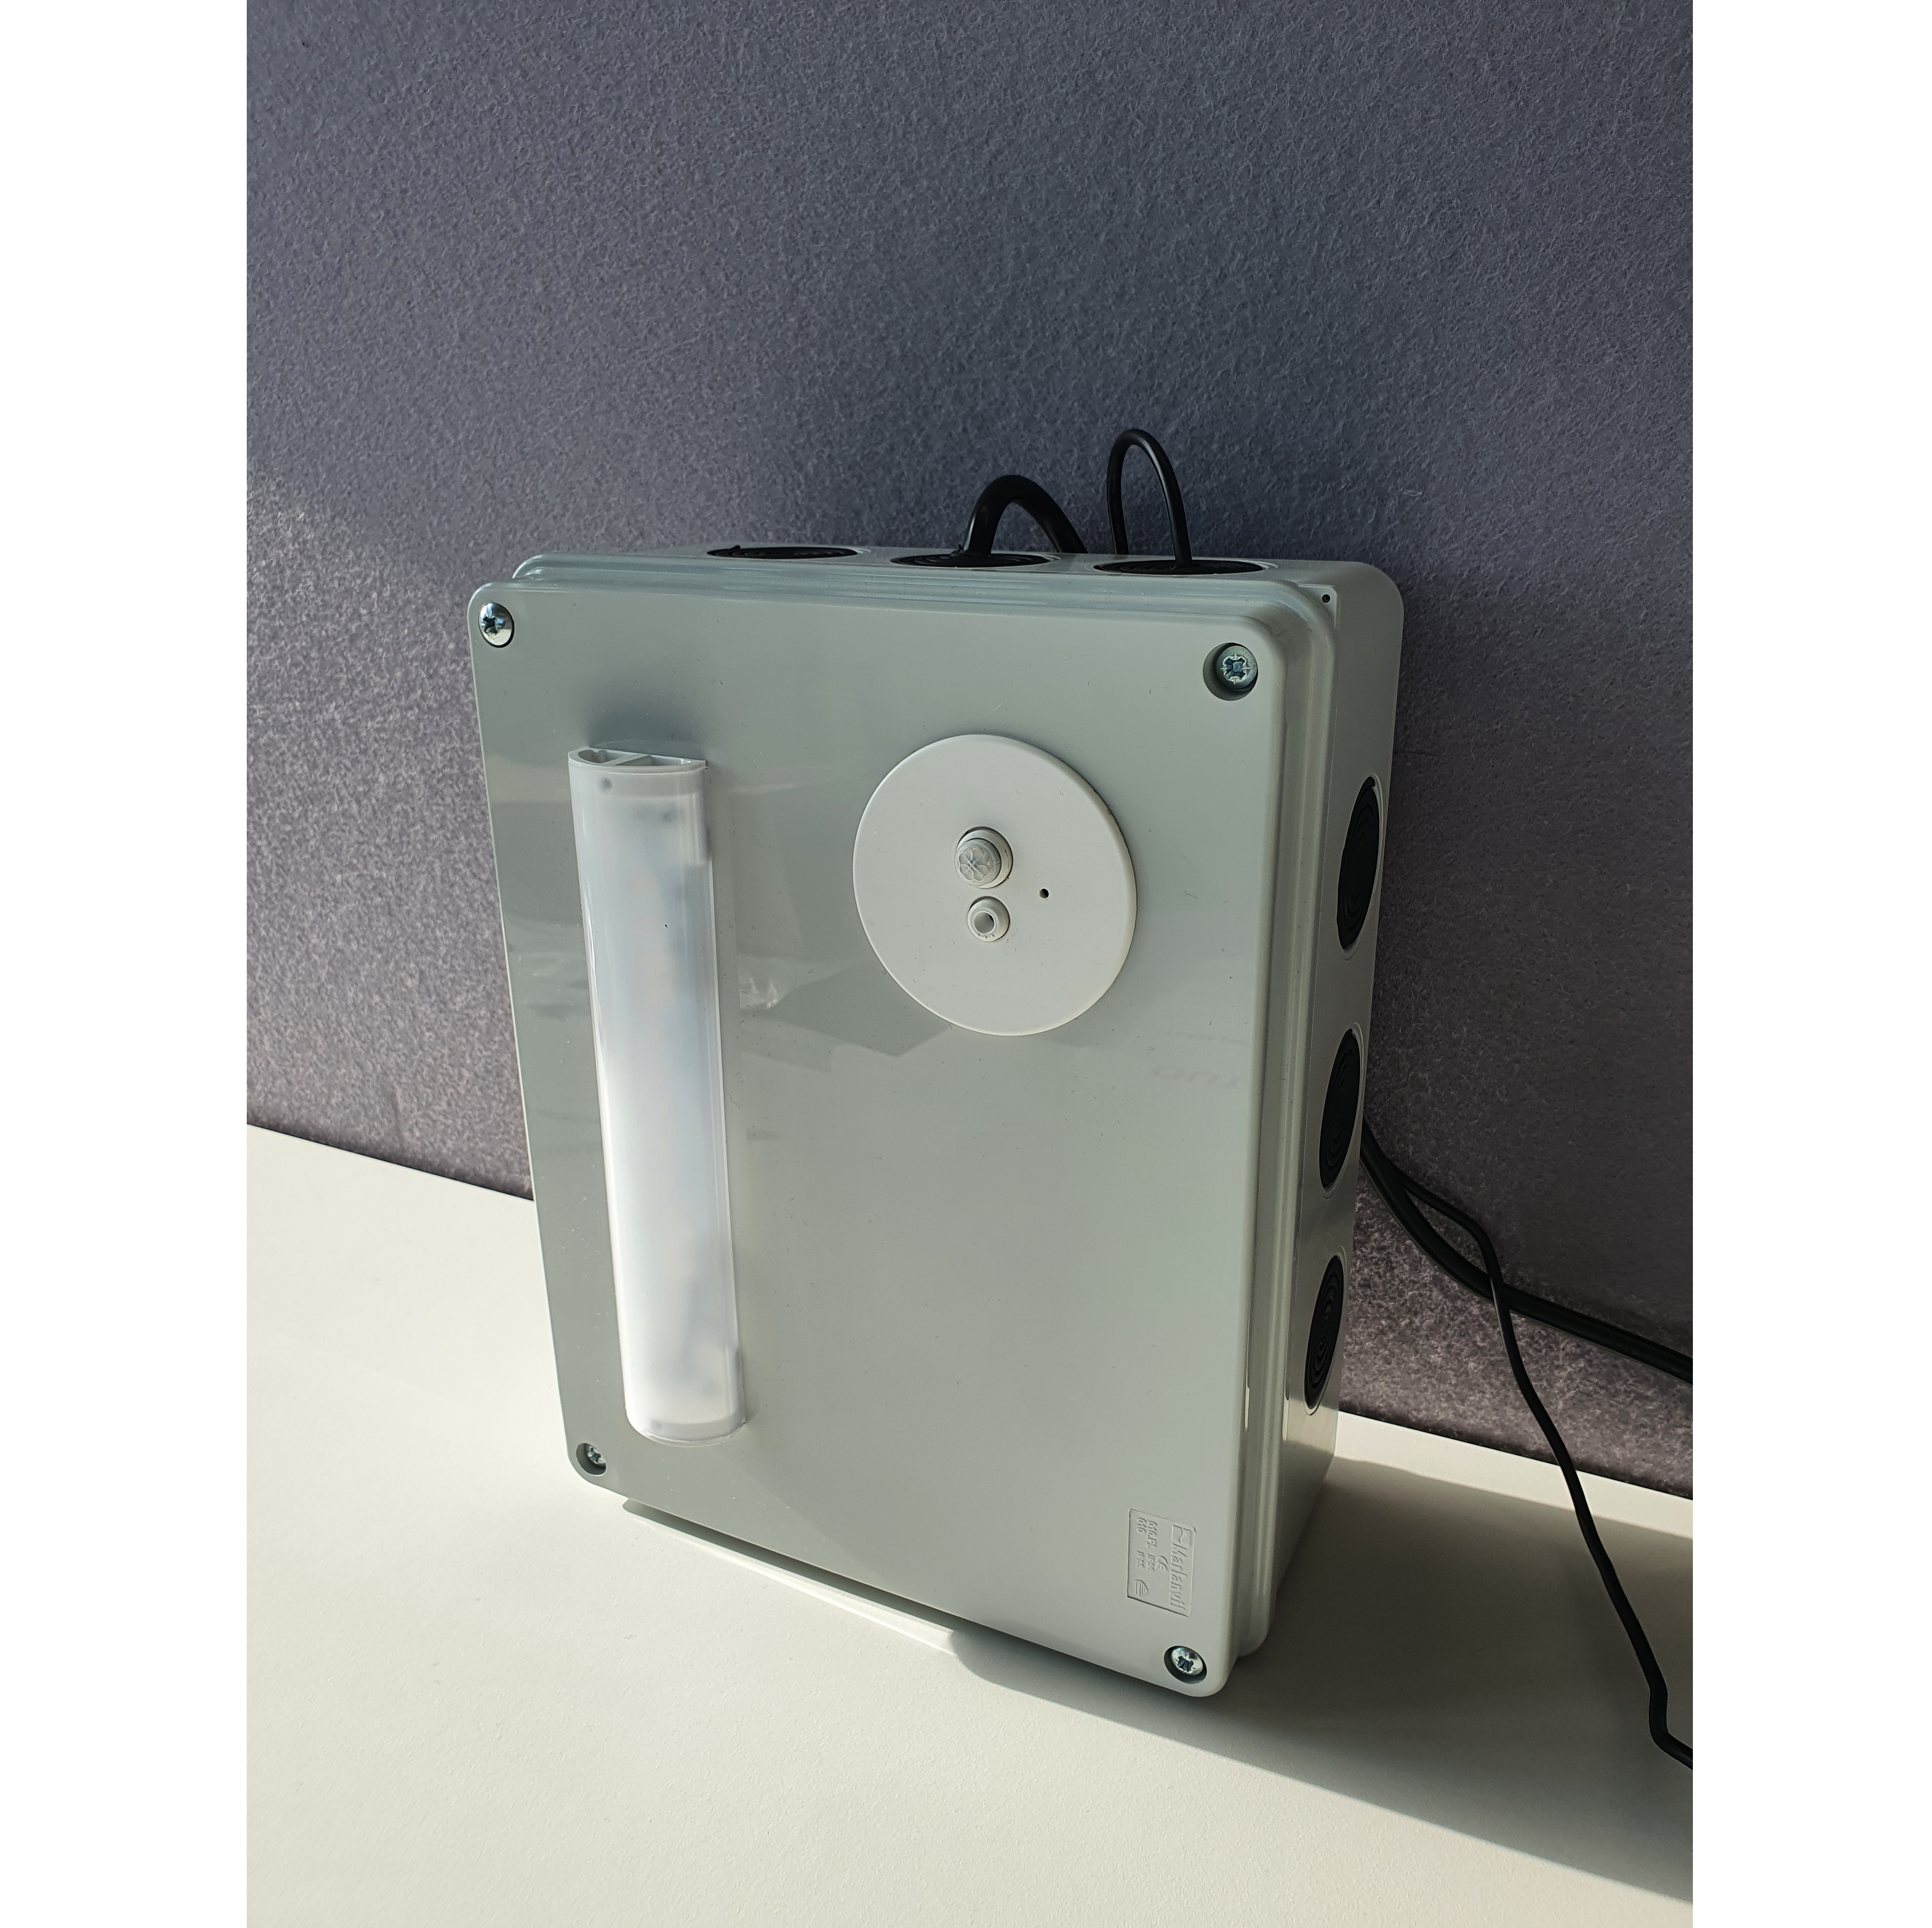
\includegraphics[width=0.5\textwidth]{thesistemplate/images/testbox_11.jpg}
    \caption{The assembled prototype for testing, LED light source attached to the left side while audio and PIR sensors to the top right part of the box.}
    \label{fig:testbox_desk}
  \end{center}
\end{figure}


For logging and data visualization additional hardware extensions and minor software modifications were necessary for the setup, given the limited amount of memory of the microcontroller and relatively difficult interfacing options with remote services. Therefore an additional Raspberry Pi 4B (rPi) was added to the box which logged the prediction confidence values with a timestamp every time it arrived from a preconfigured serial port. The extra hardware is placed to the top right part of the box, as it can be seen on \autoref{fig:testbox_inside}. The microcontroller code is altered to update the rPi each time it changes the confidence value. The rPi then saves the data incrementally to a file and streams it to an open-source cloud data visualizer for real-time status tracking.

For comparing the predictions from the prototype we need to obtain the ground truth for presence in the given meeting room and collect PIR data from the existing lighting control infrastructure. For simplicity, the ground truth was recorded manually by the author, given the fact that due to the low office usage there were only a few usages of meeting rooms per day. The ground truth contains the entry and exit time of a room occupant with one-second precision. Each testing room was equipped with a ceiling-mounted PIR sensor which constantly sends movement detection signals to the private cloud service for space usage monitoring. The actual luminaire light level can be inferred from those signals, given that the system is programmed to keep the lights on until a certain amount of time after each movement trigger. This timeout value can adjust the aggressiveness of the light control strategy and it was fixed to 6.5 minutes in our case as a typical value.


\section{Test results}

An example test sequence result corresponds to a regular working day morning is reported at \autoref{fig:light_output_comp}. As the first plot shows there were four occurrences when the phone booth was occupied for a different length ranging from a few minutes to a half an hour session approximately. Both solutions were able to sense the incoming person instantly but there were significant differences in the detection at the end of the session. PIR-only-based solutions are needed to keep the light on much longer to avoid false off decisions during a meeting due to lack of movement. This misbehavior was caught during the data collection and was indicated with gray area in the second plot. This represents a malfunction in the control process, and which period was correctly classified by the fusion sensor based solution. Most probably the algorithm prediction was reinforced by the sound information in that time interval when there was no movement registered.

\begin{figure}[ht!]
  \begin{center}
    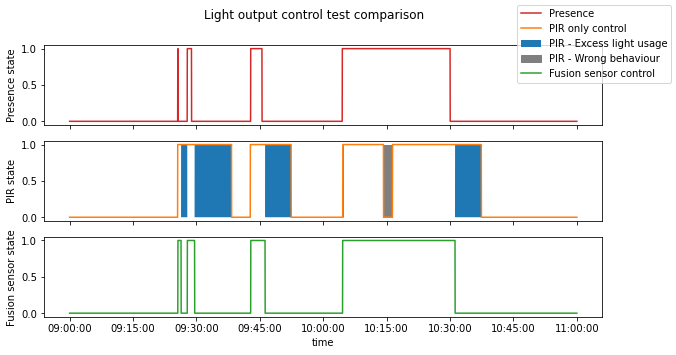
\includegraphics[width=1\textwidth]{thesistemplate/fig/light_output_control_aug23.png}
    \caption{PIR only and Multisensory light level control strategy results compared to ground truth.}
    \label{fig:light_output_comp}
  \end{center}
\end{figure}

The additional sensor allows a more aggressive turn-off policy which reduces excess energy usage in the building. The surplus which is the difference between the PIR only and the Fusion sensor based solution is indicated by the blue area in the second plot. Following the proposed approach approximately 80 \% of the excess energy could be saved by the reduction of timeout values for this particular test case.

\begin{figure}[ht!]
  \begin{center}
    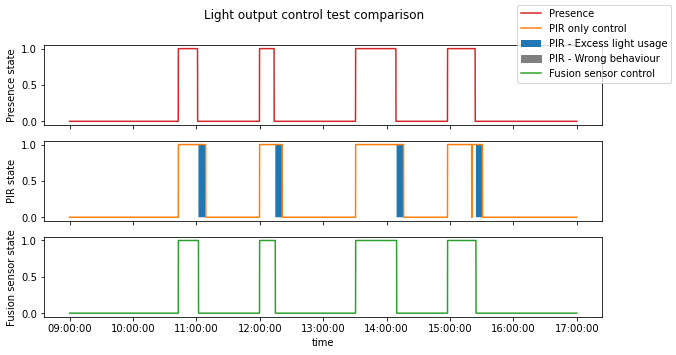
\includegraphics[width=1\textwidth]{thesistemplate/fig/light_output_control_aug27.png}
    \caption{PIR only and Multisensory light level control strategy results compared to ground truth.}
    \label{fig:light_output_comp}
  \end{center}
\end{figure}


\begin{figure}[h!]
  \begin{center}
    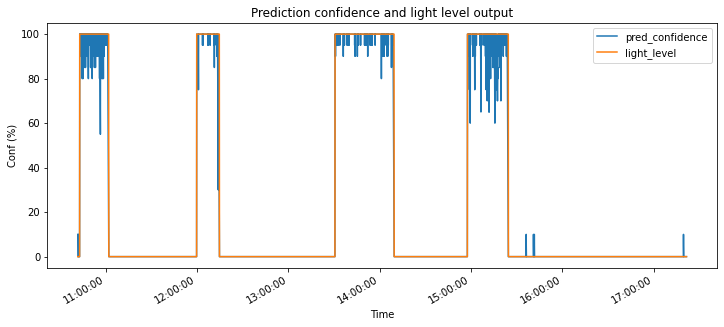
\includegraphics[width=1\textwidth]{thesistemplate/fig/conf_with_lights3.png}
    \caption{Room occupancy confidence with controlled light level values.}
    \label{fig:conf_with_lights}
  \end{center}
\end{figure}


% \begin{figure}[ht]
%     \centering
%     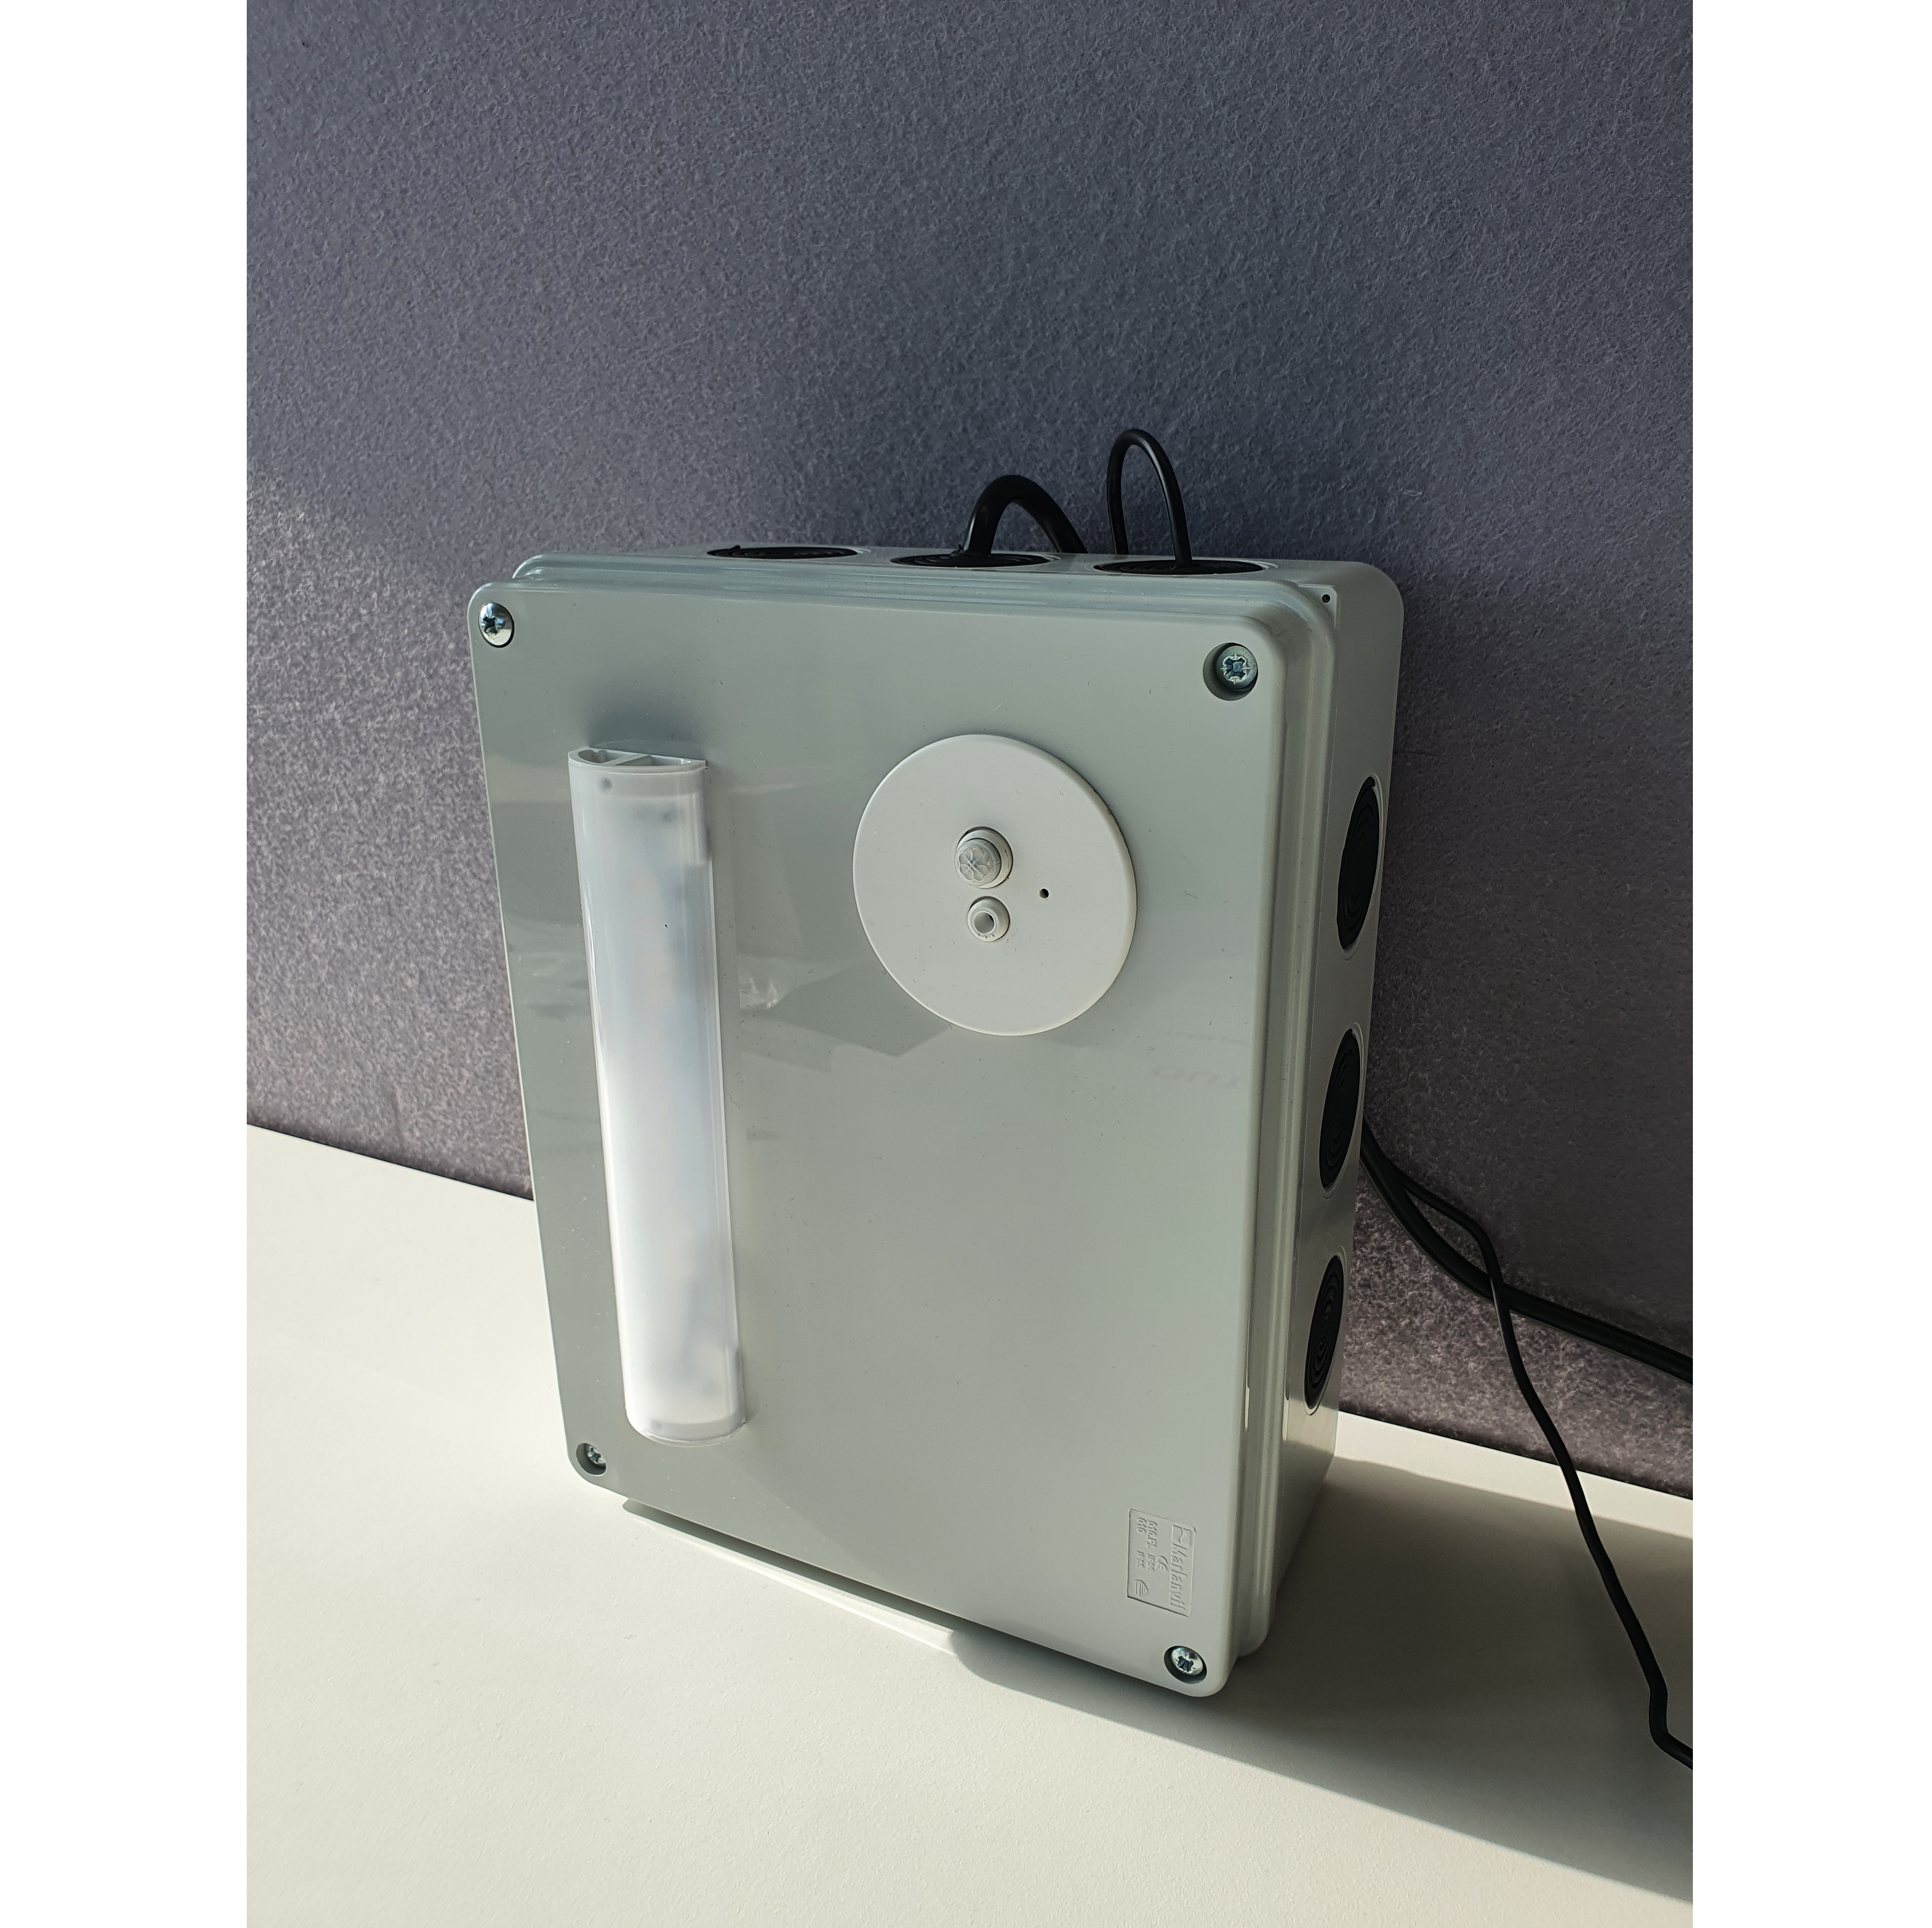
\includegraphics[width=6.5cm]{thesistemplate/images/testbox_11.jpg} 
%     %\hfill
%     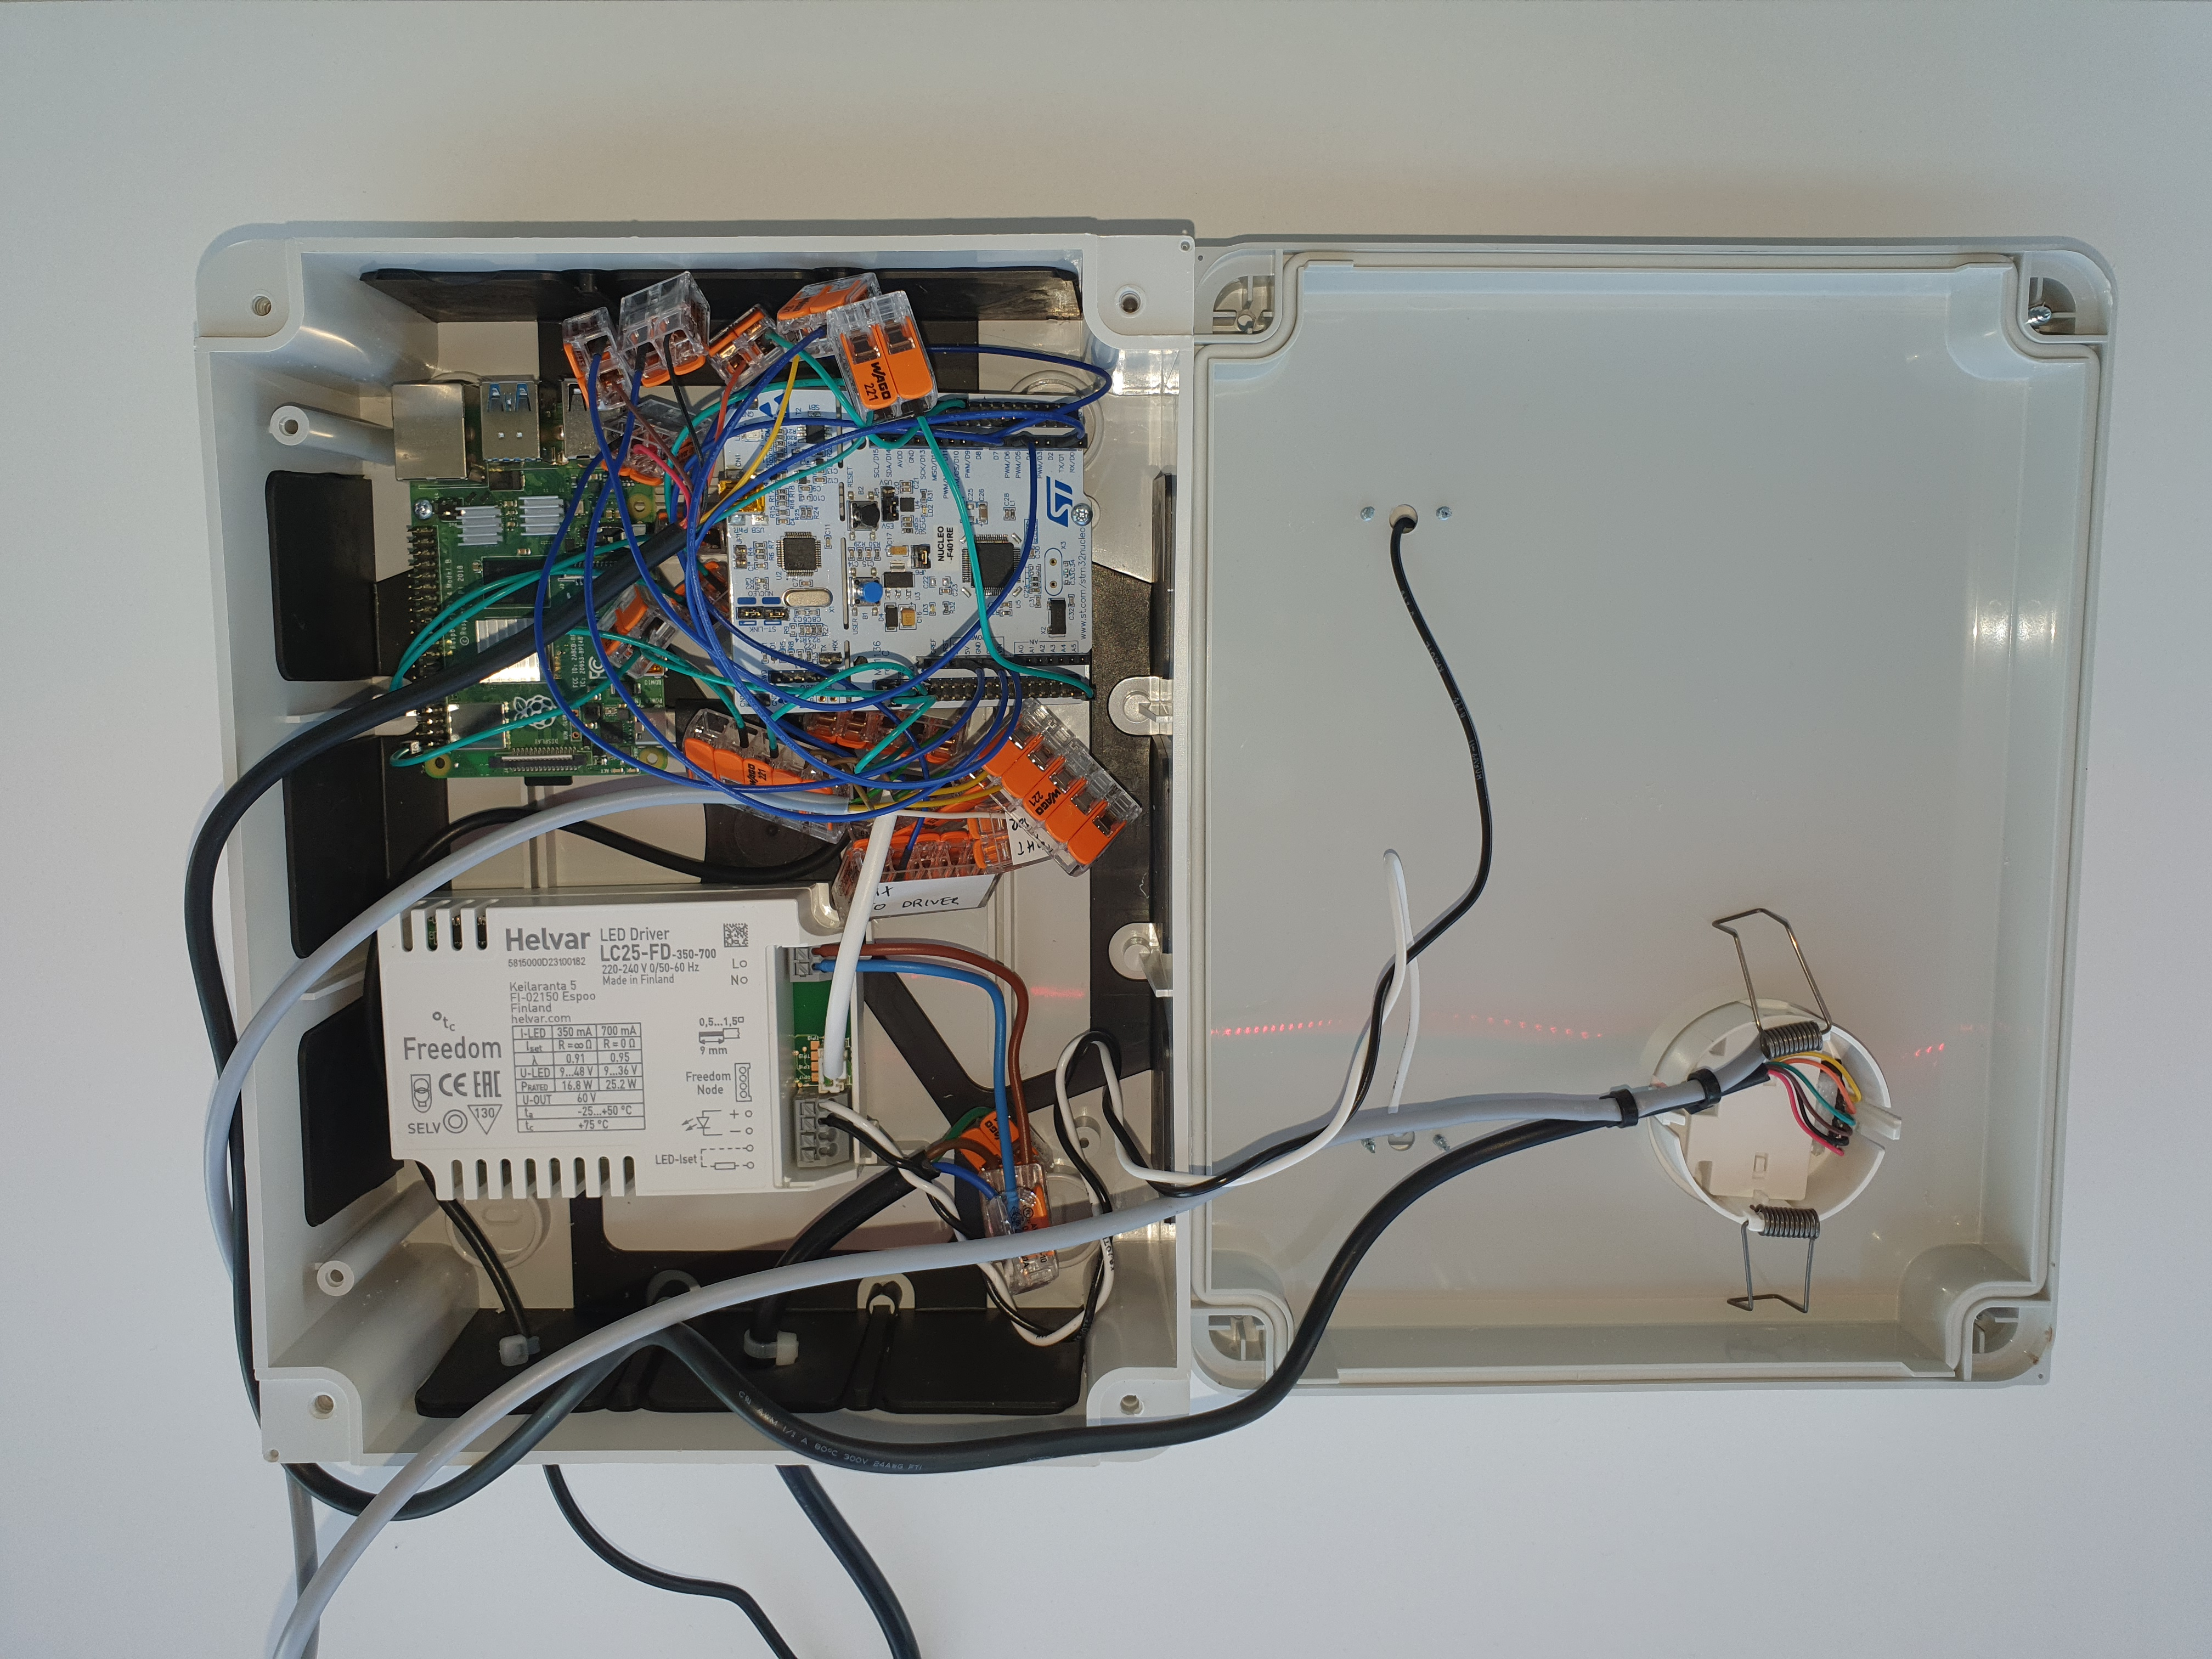
\includegraphics[width=6.5cm]{thesistemplate/images/testbox_2.jpg}
%     \caption{Inside of the prototype for multisensory room occupancy prediction, audio and PIR sensors are connected to the ST development board (white), while a Raspberry Pi 4B (green) is utilized for streaming confidence status. Small LED strip also attached to the outside, controlled by a Helvar LED-driver (white box)}
%     \label{fig:testbox}
% \end{figure}


\begin{figure}[ht!]
  \begin{center}
    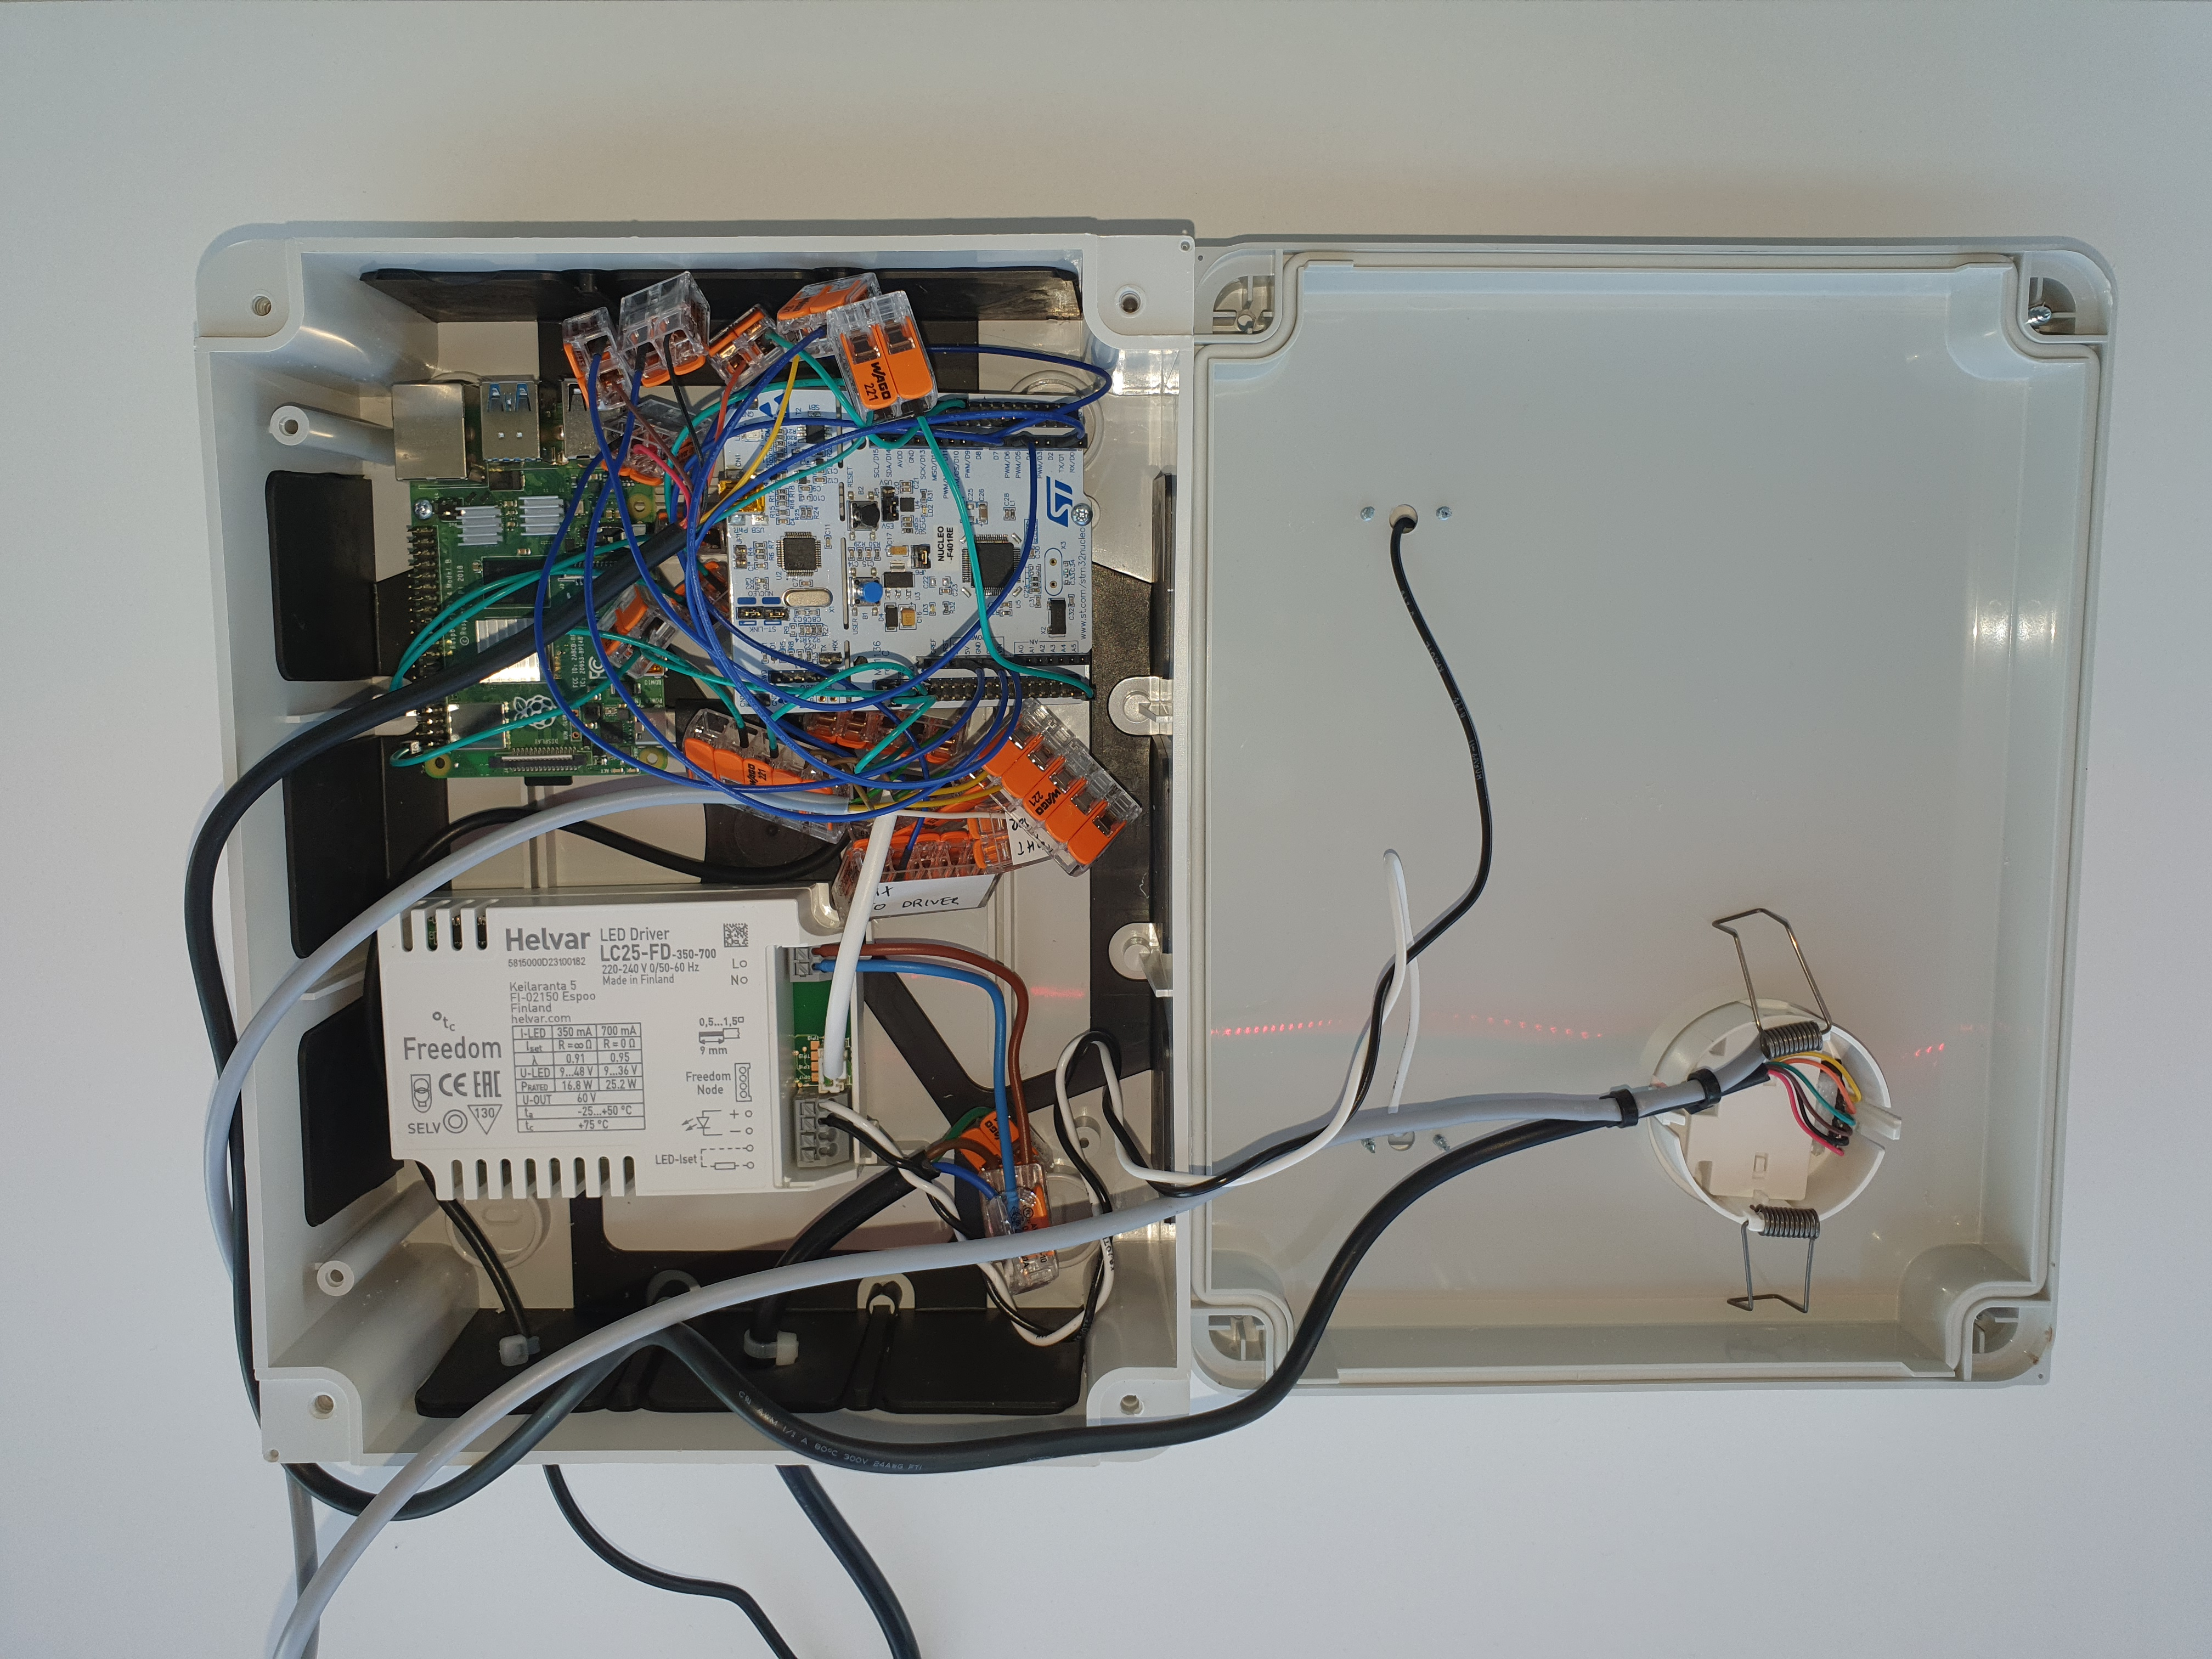
\includegraphics[width=1\textwidth]{thesistemplate/images/testbox_2.jpg}
    \caption{Inside of the prototype for multisensory room occupancy prediction, audio and PIR sensors are connected to the ST development board (white PCB), while a Raspberry Pi 4B (green PCB) is utilized for logging prediction confidence status. Small LED strip also attached to the outside, controlled by a Helvar LED-driver (white box).}
    \label{fig:testbox_inside}
  \end{center}
\end{figure}

% \begin{figure}%
%     \centering
%     \subfloat[\centering label 1]{{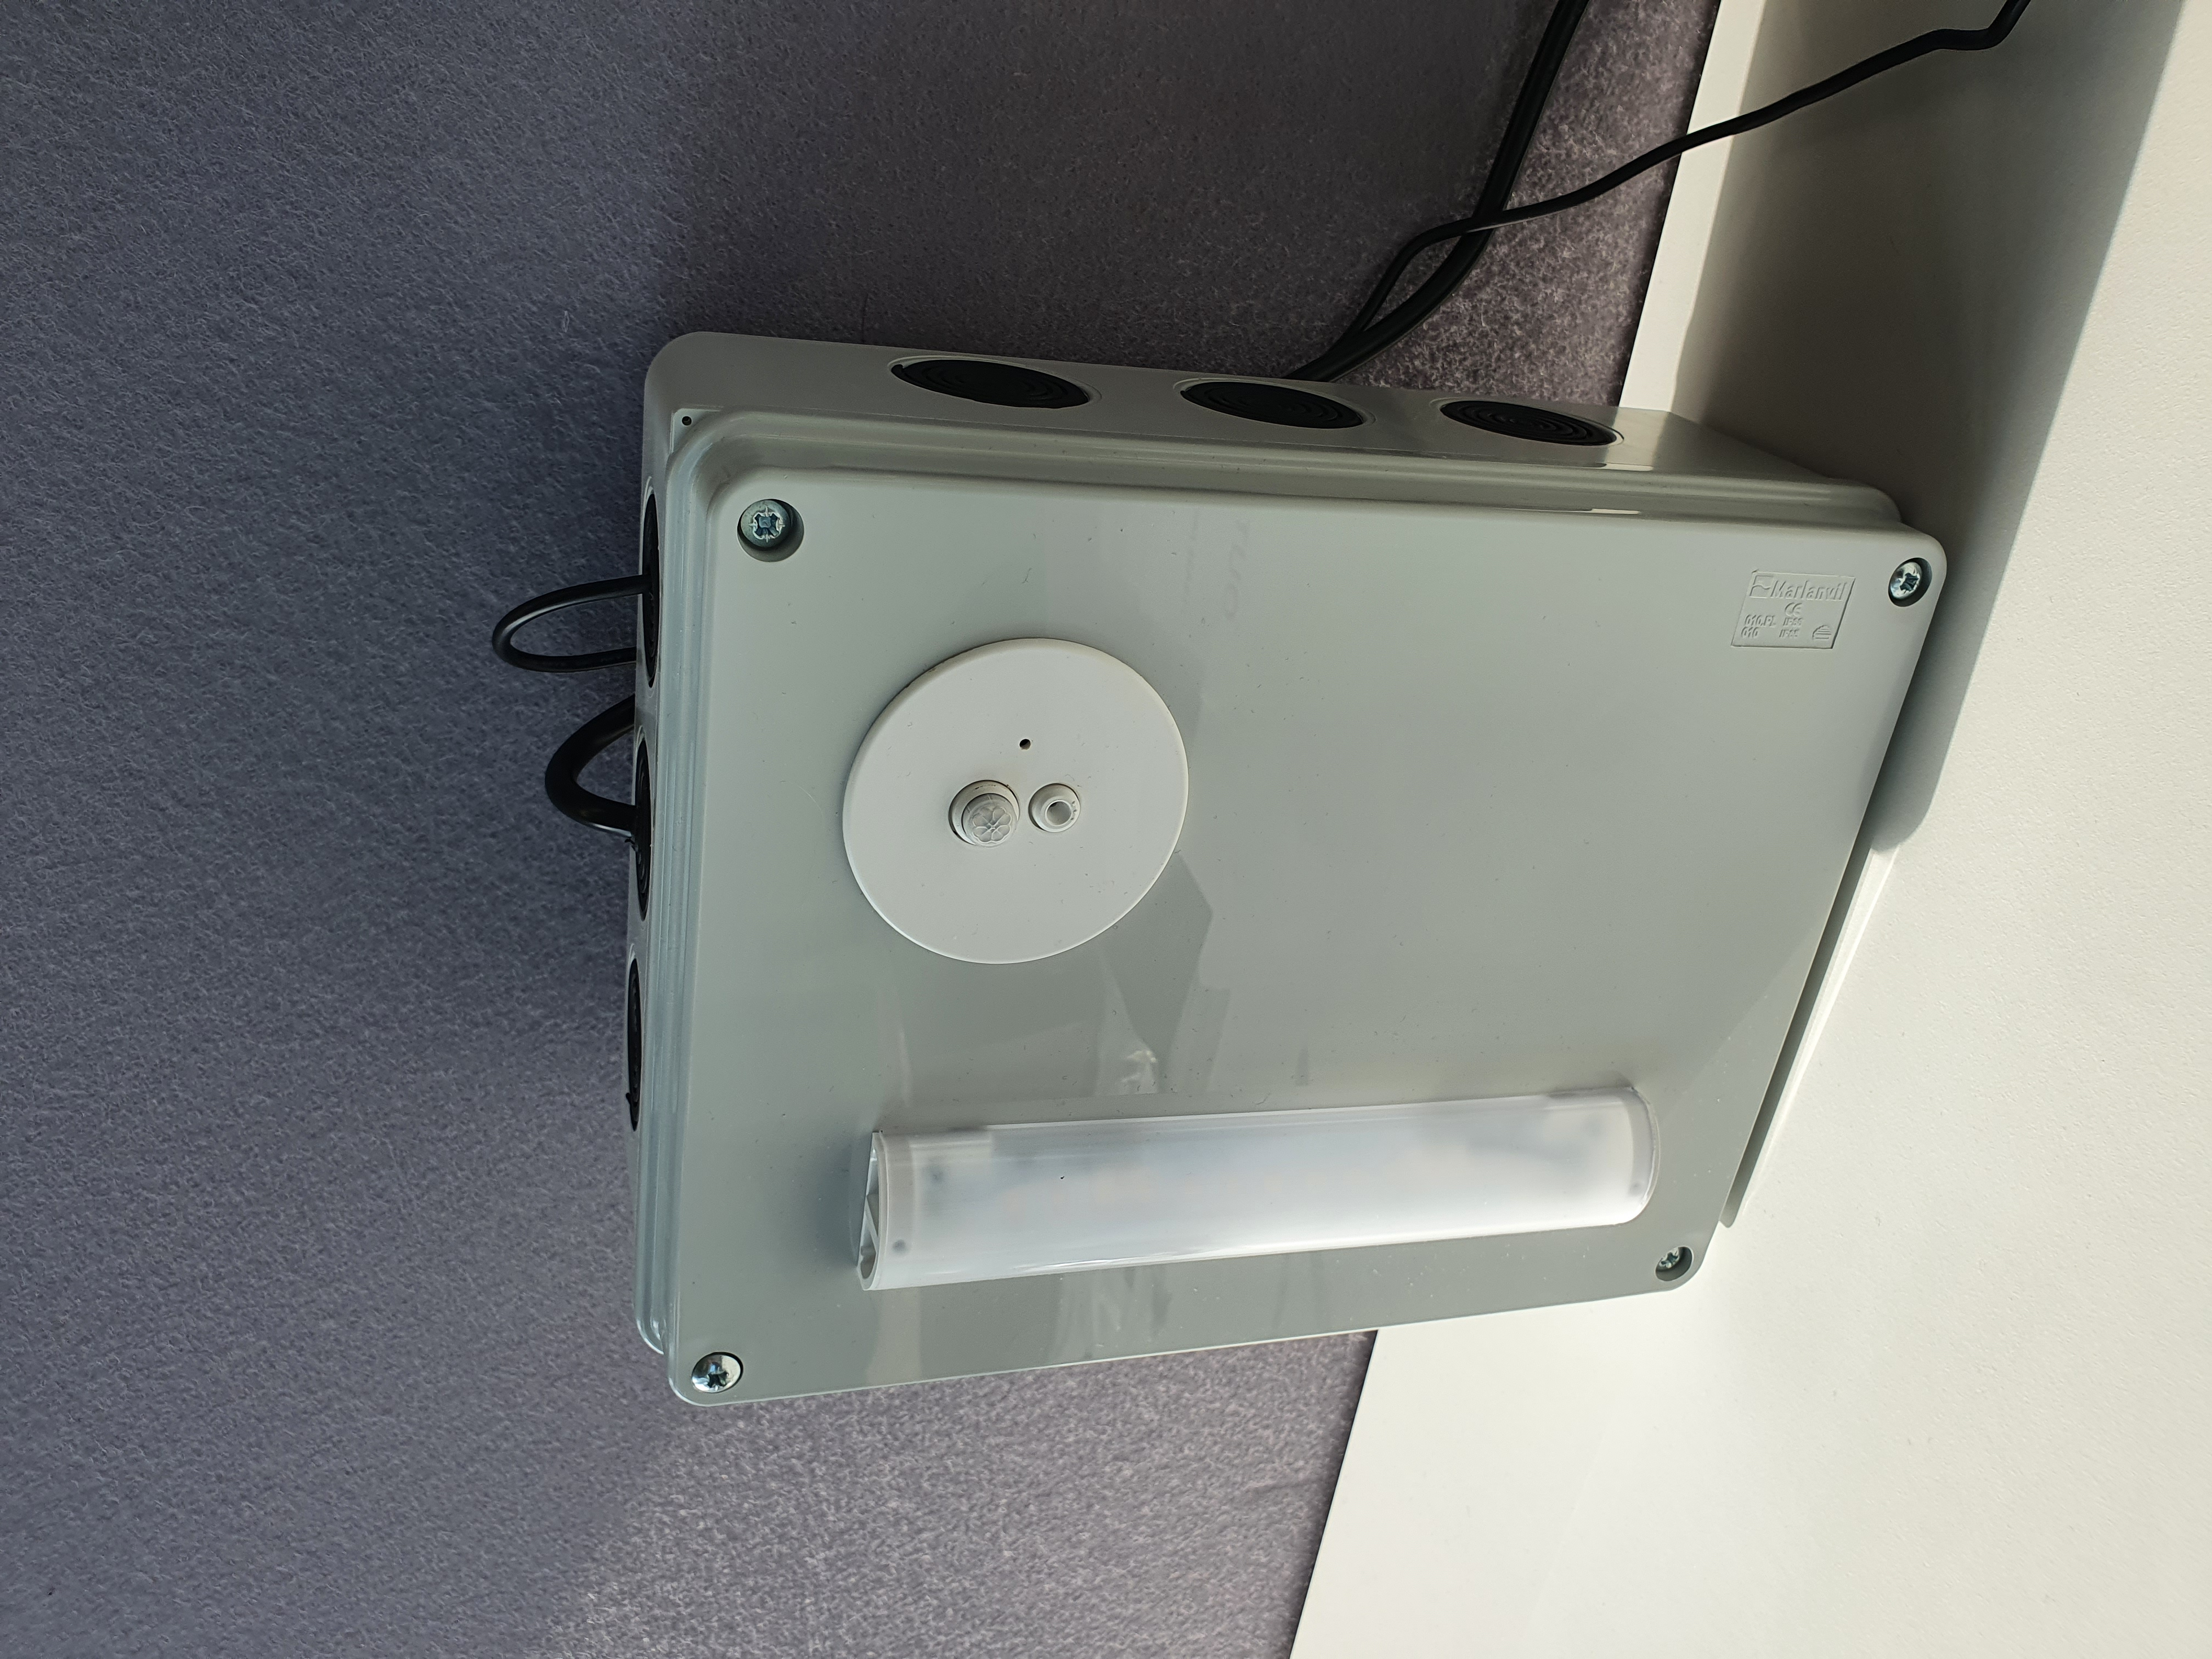
\includegraphics[width=5cm]{thesistemplate/images/testbox_1.jpg} }}%
%     \qquad
%     \subfloat[\centering label 2]{{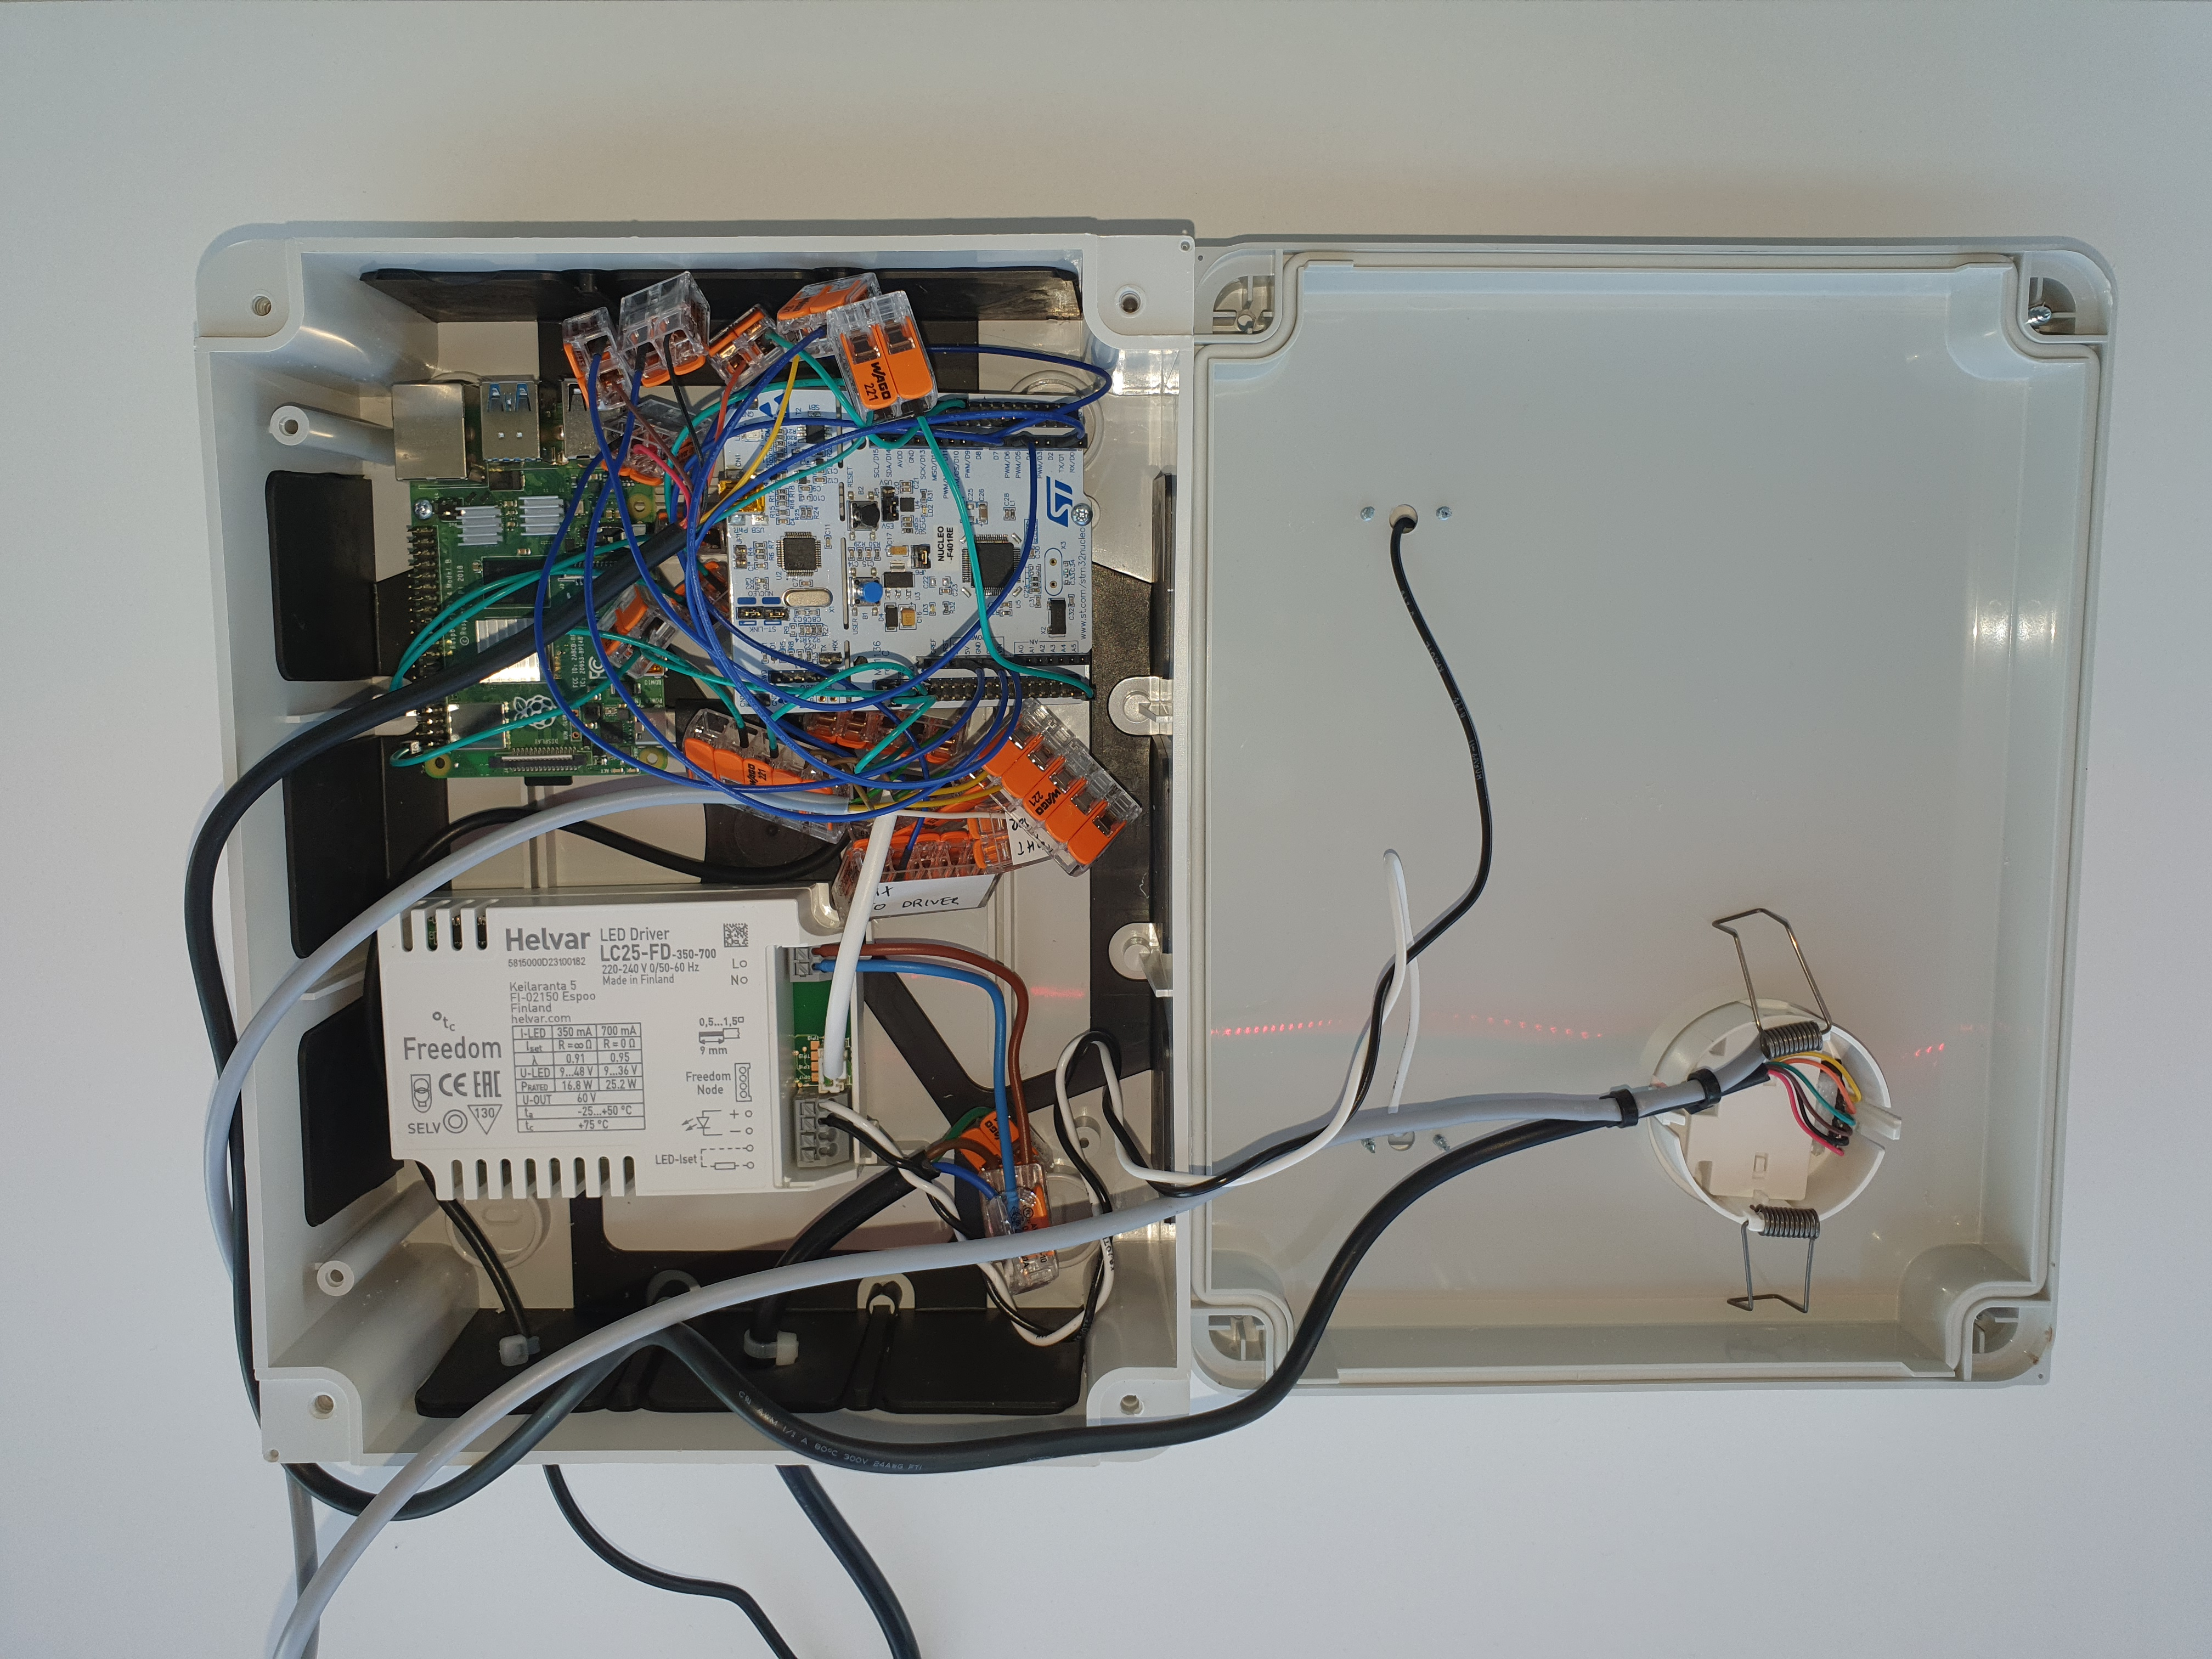
\includegraphics[width=5cm]{thesistemplate/images/testbox_2.jpg} }}%
%     \caption{2 Figures side by side}%
%     \label{fig:example}%
% \end{figure}

\section{Limitations of the used approach}

The multi-day test of the prototype has also revealed some of the weaknesses and hard limitations of the selected sensors and developed algorithms. One such extreme case is shown at \autoref{fig:light_output_faulty}. Unfortunately, the multisensory approach did also suffer from false-negative predictions and turned off the LED strip in situations where the space was occupied by an office worker. As it turned out the person did participate in a virtual meeting during the faulty light control behavior but only listened to others through a headset, leaving a minimal amount of noise or movement for the sensors. Since the current implementation applies less than 30 seconds of timeout this design choice turned to be too aggressive for this particular scenario. However, fine-tuning timeout values and adjusting weights assigned to sensor outputs are outside of the scope of the thesis, since it would require a more thorough analysis of the various use cases.




\begin{figure}[ht!]
  \begin{center}
    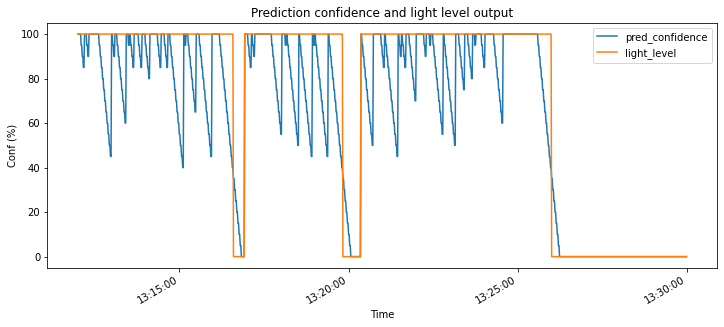
\includegraphics[width=1\textwidth]{thesistemplate/fig/light_output_control_bad.png}
    \caption{Malfunctioning light level control scenario, while room occupancy. The quick jumps back to 100\% are due to PIR triggers, but there is only little reinforcement from sound, which makes the timeout value too short and producing False Negative predictions. }
    \label{fig:light_output_faulty}
  \end{center}
\end{figure}
